%% Beispiel-Präsentation mit LaTeX Beamer im KIT-Design
%% entsprechend den Gestaltungsrichtlinien vom 1. August 2020
%%
%% Siehe https://sdqweb.ipd.kit.edu/wiki/Dokumentvorlagen

%% Beispiel-Präsentation
\documentclass[en]{sdqbeamer} 

%% Footnote without numbering
\newcommand\nonumberfootnote[1]{%
  \begingroup
  \renewcommand\thefootnote{}\footnote{#1}%
  \addtocounter{footnote}{-1}%
  \endgroup
}
 
%% Titelbild
\titleimage{banner_2020_kit}

%% Gruppenlogo
\grouplogo{} 

%% Gruppenname und Breite (Standard: 50 mm)
\groupname{Institute for Automation and Applied Informatics (IAI)}
\groupnamewidth{60mm}

% Beginn der Präsentation

\title[ABAC for Substations]{Certificateless Attribute-Based Server-Aided Cryptosystem\\for Substation Automation Systems (CASC-SAS)}
\subtitle{Master's Thesis Mid-Term Presentation} 
\author[Moritz Gstuer]{Moritz Gstuer}

\date[31.\,10.\,2024]{31. October 2024}

% Literatur 
 
\usepackage[citestyle=authoryear,bibstyle=numeric,hyperref,backend=biber]{biblatex}
\addbibresource{../bibliography/masterthesis.bib}
\bibhang1em

\begin{document}
 
%Titelseite
\KITtitleframe

%Inhaltsverzeichnis
\begin{frame}{Agenda}
\tableofcontents
\end{frame}

\section{Motivation}
\begin{frame}{Motivation}
    \centering
	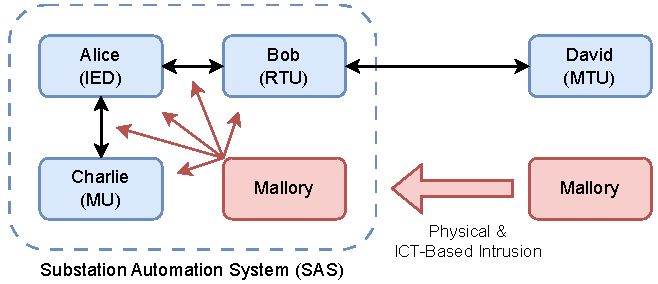
\includegraphics[width=0.8\textwidth]{./figures/sas_intrusion.drawio.pdf}
    \nonumberfootnote{IED\dots Intelligent Electronic Device | MU\dots Merging Unit | RTU\dots Remote Terminal Unit}
    \nonumberfootnote{MTU\dots Master Terminal Unit | ICT\dots Information and Communications Technology}
\end{frame}
\begin{frame}{SAS Communication: Requirements \& Constraints}
    \begin{blueblock}{Requirements}
        \begin{itemize}
            \item Integrity
            \item Authenticity
            \item Non-Repudiation
            \item Least Privilege Principle (PoLP)
            \item Separation of Duties (SoD)
        \end{itemize}
        $\rightarrow$ Authentication, Authorization, \& Access Control
    \end{blueblock}
    \begin{grayblock}{Constraints: IEC 61850 Message Types \& Performance Classes \parencite*{IEC61850P5,IEC61850P8}}
        Client-Server (Unicast) \& Publisher-Subscriber (Broadcast/Multicast) \\$\rightarrow$ Resource \& Time Constraints!
        \\Examples: GOOSE (Type 1A, 3 ms), SV (Type 4, 3 ms), MMS (Type 2/3/5, 100-10000 ms)
    \end{grayblock}
\end{frame}

\begin{frame}{Research Questions}
    \begin{greenblock}{Authorization \& Access Control in SAS}
        How can expressive and flexible but yet computationally expensive access control be employed in a SAS?
        \\$\rightarrow$ Real-Time Attributes, Ad-Hoc Policy Evaluation, \& Speedup Solutions
    \end{greenblock}

    \begin{greenblock}{Public-Key Cryptography in SAS}
        How can a secure and lightweight public-key approach be designed, implemented, \& employed in a SAS?
        \\$\rightarrow$ (Dis-)Advantages, \& Speedup Solutions
    \end{greenblock}

    \begin{greenblock}{Security Architecture for Time-Critical Communication}
        How can authentication, authorization, and access control be integrated into a malleable, scalable, and lightweight cryptosystem for time-critical SAS communication?
        \\$\rightarrow$ System Model, Domain Requirements, Architecture, \& Protocols
    \end{greenblock}
\end{frame}

\section{Approach}
\begin{frame}{CASC-SAS Approach}
    \begin{greenblock}{\textbf{C}ertificateless \textbf{A}ttribute-Based \textbf{S}erver-Aided \textbf{C}ryptosystem for \textbf{S}ubstation \textbf{A}utomation \textbf{S}ystems (CASC-SAS)}
        \begin{itemize}
            \item \textbf{S}erver-Aided \textbf{A}ttribute-\textbf{B}ased \textbf{A}uthorization \& \textbf{A}ccess \textbf{C}ontrol (SABAAC)
            \item \textbf{C}ertificateless \textbf{A}ttribute-Based \textbf{S}erver-Aided \textbf{A}uthentication (CASA)
        \end{itemize}
    \end{greenblock}
\end{frame}
\begin{frame}{Authentication, Authorization, \& Access Control}
    \begin{redblock}{Problem: Policy Evaluation Complexity}
        Fine-grained \& flexible access control relying on dynamic authorization \& authentication
        \\$\rightarrow$ Ad-hoc evaluation in real-time environment
    \end{redblock}

    \begin{greenblock}{Solution: Server-Aided Access Control}
        Delegation of authorization \& access control to semi-trusted server (PDP)
        \\$\rightarrow$ Authentication at each device (server-aided)
        \\$\rightarrow$ Speedup Techniques: Evaluation pre-computation \& access decision caching
    \end{greenblock}

    \begin{grayblock}{Architecture \parencite{Hu2014,Oasis2013}}
        \begin{itemize}
            \item Policy Decision Point (PDP) $\rightarrow$ Computes access decisions by evaluating policies
            \item Policy Enforcement Point (PEP) $\rightarrow$ Enforces policy decisions by controlling access to protected objects
        \end{itemize}
    \end{grayblock}
\end{frame}
\begin{frame}{CASC-SAS Architecture: Function-Oriented}
    \centering
    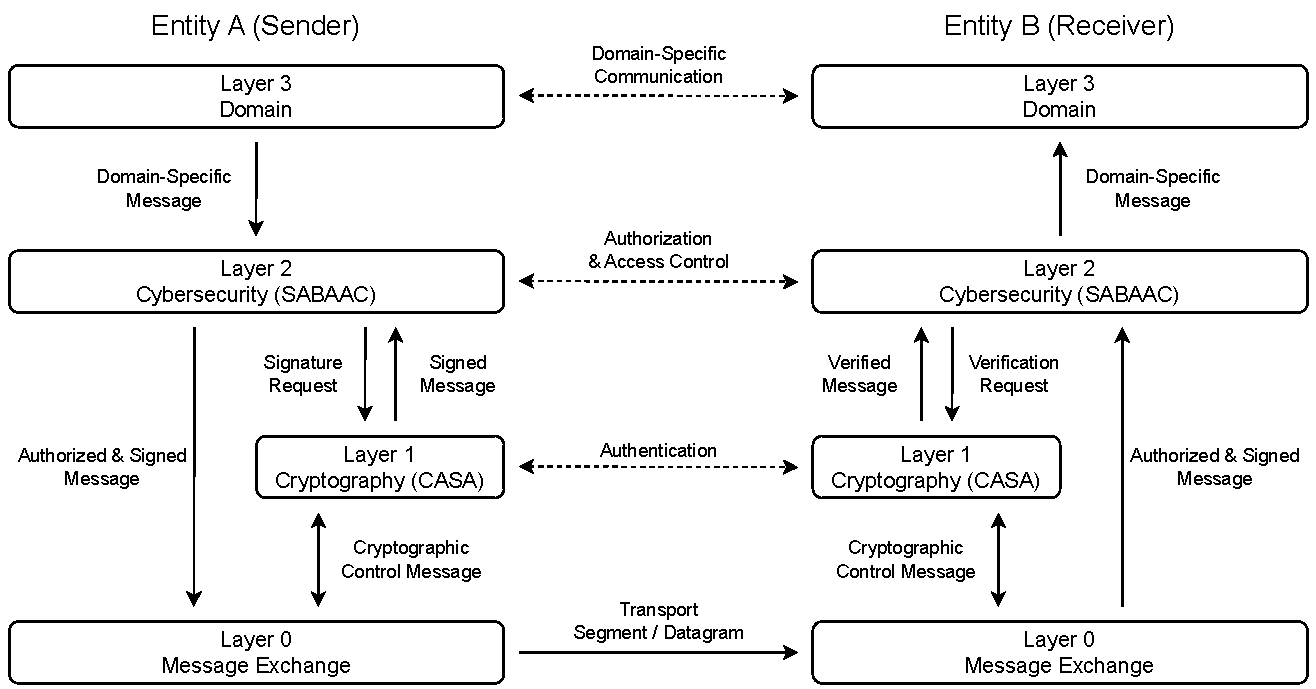
\includegraphics[height=0.75\textheight]{./figures/layers_request_example.drawio.pdf}
\end{frame}
\begin{frame}{CASC-SAS Architecture: Component-Oriented}
    \begin{columns}
        \column{.7\textwidth}
        \centering
        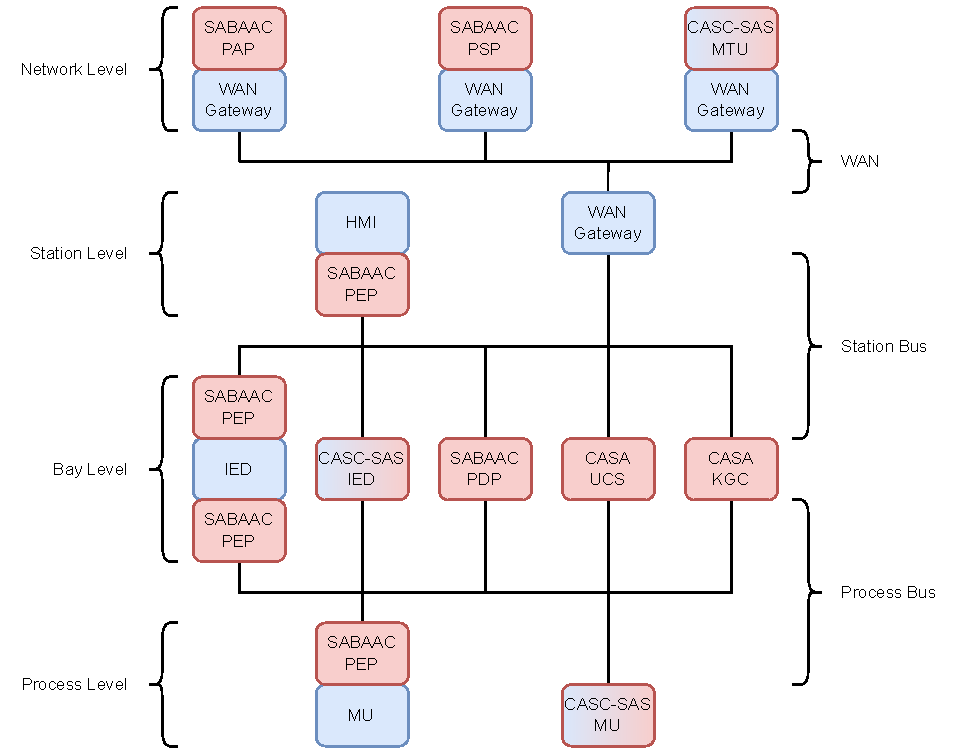
\includegraphics[height=0.75\textheight]{./figures/casc_architecture_color.drawio.pdf}
        \column{.3\textwidth}
        \footnotesize
        HMI\dots Human-Machine Interface\\IED\dots Intelligent Electronic Device\\KGC\dots Key Generation Center\\MTU\dots Master Terminal Unit\\MU\dots Merging Unit\\PAP\dots Policy Administration Point\\PDP\dots Policy Decision Point\\PEP\dots Policy Enforcement Point\\PSP\dots Policy Storage Point\\RTU\dots Remote Terminal Unit\\UCS\dots Untrusted Cryptography Server\\WAN\dots Wide Area Network
    \end{columns}
\end{frame}

\section{Work Plan}
\begin{frame}{Work in Progress}
    \begin{blueblock}{Milestone: Realization}
        \textbf{Finished:} Local authentication, delegated authorization, \& delegated access control protocol 
        \\\textbf{In Progress:}  Server-aided authentication via own signature scheme, \& policy DSL
        \\$\rightarrow$ Currently: $\sim$3100 SLOC, object-oriented, Java 17 \& Kotlin
        \\$\rightarrow$ Planned: $\sim$5000 SLOC, published open-source
    \end{blueblock}
    \begin{blueblock}{Milestone: Evaluation}
        \textbf{Finished:} Testbed construction \& preliminary performance results
        \\\textbf{In Progress:} Evaluation of performance, security, \& compatibility
        \\$\rightarrow$ Planned: Code \& results of experiments published open-source
    \end{blueblock}
\end{frame}
\begin{frame}{What's next?}
    \begin{blueblock}{Milestone: Conclusion}
        Limitations, future work, \& summary of thesis
    \end{blueblock}
    \begin{blueblock}{Milestone: Review \& Finalization}
        \textbf{Thesis:} Proofreading, review, printing, \& binding 
        \\\textbf{Final Presentation:} Preparation, proofreading, \& review
    \end{blueblock}
    \begin{redblock}{Estimated Time of Completion (ETC)}
        \textbf{Draft:} November 25, 2024
        \\\textbf{Final:} January 01, 2025
        \\\textbf{Deadline:} February 03, 2025
    \end{redblock}
\end{frame}

\section{Evaluation}
\begin{frame}{Performance Evaluation}
    \begin{greenblock}{Question}
        Is CASC-SAS capable of securing time-constrained communication of a SAS?
        \\$\rightarrow$ Computational complexity, supported message types, \& network exception resilience
    \end{greenblock}
    \begin{blueblock}{Approach}
        Experimentally performed evaluation based on realization
        \\$\rightarrow$ Currently: Testbed-based experiments
        \\$\rightarrow$ Planned: Lab-based experiments
    \end{blueblock}
\end{frame}
\begin{frame}{Preliminary Results}
    \centering
    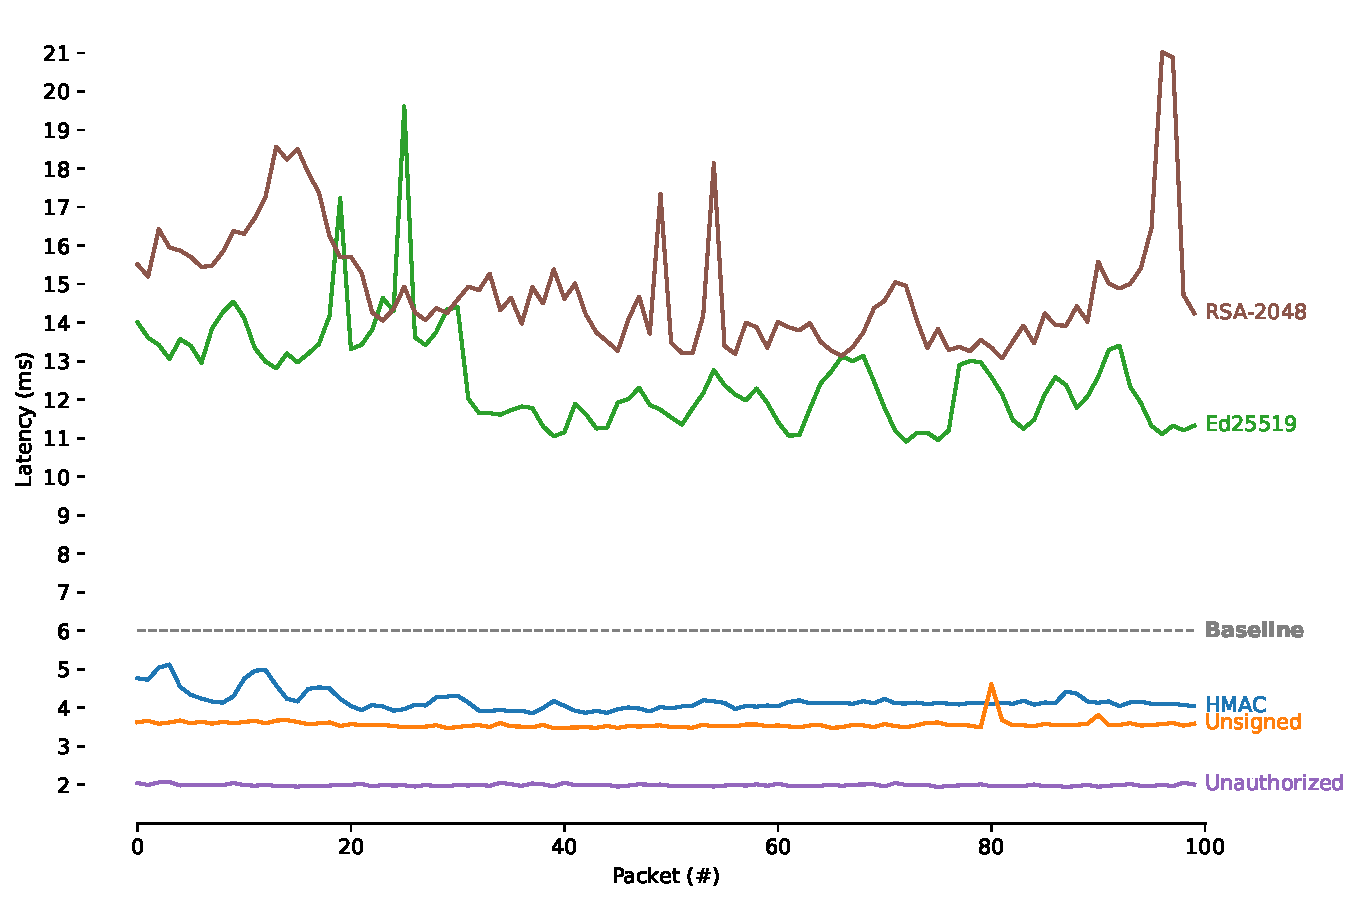
\includegraphics[height=0.78\textheight]{./figures/rtt-estimation-results.pdf}
\end{frame}
\begin{frame}{Discussion: 10k Sequential Packets}
    \begin{blueblock}{Access Control Overhead}
        \begin{tabular}{r r r r}
            & \multicolumn{1}{c}{Avg} & \multicolumn{1}{c}{Min} & \multicolumn{1}{c}{Throughput}\\
            \textbf{Unauthorized} & 2.0 ms & 1.7 ms & 465 PPS\\
            \textbf{Unsigned} & 3.3 ms & 2.8 ms & 292 PPS
        \end{tabular}
        %\textbf{Unauthorized:} $\sim$2.0 ms RTT (min $\sim$1.7 ms) 465 PPS
        %\\\textbf{Unsigned:} $\sim$3.3 ms RTT (min $\sim$2.8 ms) 292 PPS
        \vspace{0.5em}
        \\$\rightarrow$ Access Control: +1.3 ms RTT (+65 \%)
    \end{blueblock}
    \begin{blueblock}{Authentication Overhead}
        \begin{tabular}{r r r r}
            & \multicolumn{1}{c}{Avg} & \multicolumn{1}{c}{Min} & \multicolumn{1}{c}{Throughput}\\
            \textbf{HMAC} & 3.4 ms & 2.9 ms & 285 PPS\\
            \textbf{Ed25519} & 12.0 ms & 9.6 ms & 82 PPS\\
            \textbf{RSA-2048} & 14.0 ms & 11.4 ms & 68 PPS
        \end{tabular}
        %\textbf{HMAC:} $\sim$3.4 ms RTT (min $\sim$2.9 ms) 285 PPS
        %\\\textbf{Ed25519:} $\sim$12.0 ms RTT (min $\sim$9.6 ms) 82 PPS
        %\\\textbf{RSA-2048:} $\sim$14.0 ms RTT (min $\sim$11.4 ms) 68 PPS
        \vspace{0.5em}
        \\$\rightarrow$ Authentication: +0.1--10.7 ms RTT (+3--325 \%)
    \end{blueblock}
\end{frame}

\section{Conclusion}
\begin{frame}{Conclusion}
    \begin{redblock}{Problem}
        Current IT cyberattack mitigation approaches: Not applicable to the SAS domain!
        \\$\rightarrow$ Constraints: Resources, time, \& communication patterns
    \end{redblock}
    \begin{blueblock}{Contribution}
        CASC-SAS Security Architecture \& Framework\dots
        \\\dots employs mandatory authentication, authorization, \& access control
        \\\dots for time-critical SAS communication
        \\\dots in time-variable SAS environment.
    \end{blueblock}
    \vspace{0.5em}
    \centering
    \huge
    Thank you!
\end{frame}

\appendix
\beginbackup
\section{System Model}
\begin{frame}{Motivation}
    \begin{columns}
        \column{.4\textwidth}
        \centering
        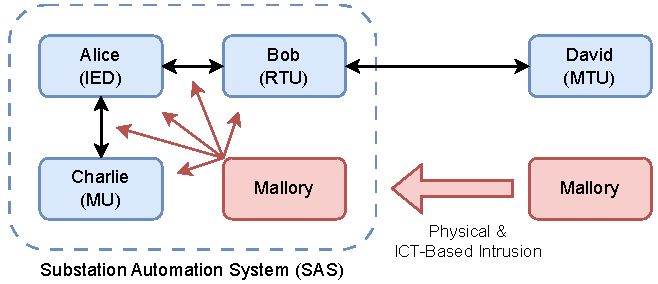
\includegraphics[width=1.0\textwidth]{./figures/sas_intrusion.drawio.pdf}
        \column{.6\textwidth}
        \begin{redblock}{Substation Threats \& Attacks}
            \begin{itemize}
                \item Eavesdropping
                \item Man-in-the-Middle
                \item Spoofing/Masquerading
                \item Replay
                \item Denial of Service\\$\rightarrow$ Flooding, Broadcast/Multicast Storm, \& Poisoning
                \item False Data Injection\\$\rightarrow$ Forged Sensor Data \& Commands, \& Configuration Tampering
            \end{itemize}
            % $\rightarrow$ Authentication, Authorization, Access Control, \& Encryption of Substation Communication
        \end{redblock}
    \end{columns}
\end{frame}
\begin{frame}{System Model: Substation Automation System (SAS)}
    \centering
    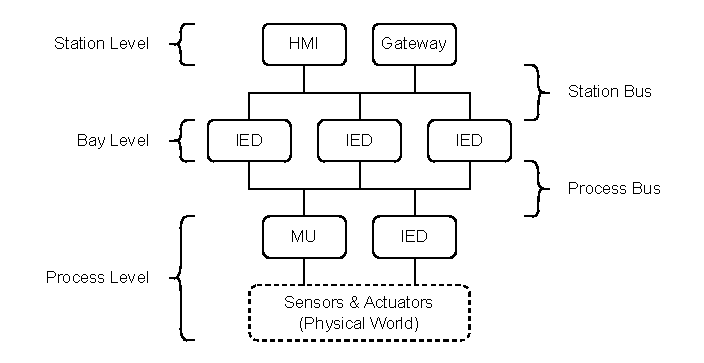
\includegraphics[width=0.7\textwidth]{./figures/substation_architecture.drawio.pdf}
    \nonumberfootnote{IED\dots Intelligent Electronic Device | MU\dots Merging Unit | HMI\dots Human-Machine Interface}
\end{frame}

\section{Related Work}
\begin{frame}{Related Work}
    \begin{blueblock}{IEC 62351 \parencite*{IEC62351P6,IEC62351P8}}
        Standard for Cybersecurity: Energy-Related Systems \& Communication Networks
        \\$\rightarrow$ Authenticity \& Integrity: Mandatory Symmetric Authentication
        \\$\rightarrow$ Confidentiality: Optional (Non-Recommended) Symmetric Encryption
        \\$\rightarrow$ Access Control: Role-Based Access Control (RBAC) (Access-Token-Driven, 7 Mandatory Roles)
    \end{blueblock}
\end{frame}
\begin{frame}{Related Work}
    \begin{blueblock}{Secure Communication in Substations}
        \begin{itemize}
            \item Bump-in-the-Wire Security Filter for GOOSE/SV MAC Tagging \& Verification \parencite{Ishchenko2018}
            \item Domain-Based Collaborative Cyberattack Mitigation Approach \parencite{Hong2019}
            \item Fixed-Latency Hardware Architecture for GOOSE/SV Encryption \& Authentication \parencite{Rodriguez2021}
        \end{itemize}
    \end{blueblock}

    \begin{blueblock}{Role-Based Access Control (RBAC) in Substations}
        \begin{itemize}
            \item XACML-Based RBAC Approach for IEC 61850 \& IEC 62351 compliant SAS \parencite{Lee2015}
            \item Distributed RBAC for Subscription-Based Remote Network Services \parencite{Ma2006} % Constraint-Enabled 
            \item Rule-Based RBAC Policy Enforcement Architecture \parencite{Alcaraz2016} % for Smart Grid Systems
        \end{itemize}
    \end{blueblock}
\end{frame}
\begin{frame}{Related Work}
    \begin{blueblock}{Attribute-Based Access Control (ABAC) in Substations}
        \begin{itemize}
            \item Firewall for Attribute-Based Access Control in Smart Grids \parencite{Ruland2018}
            \\$\rightarrow$ Firewall with XACML-Based ABAC Policies
            \\$\rightarrow$ Outer \& Inner Station Bus
            \\$\rightarrow$ Unobstructed Fast Messages (e.g. GOOSE)
            \item T-ABAC: An attribute-based access control model for real-time availability in highly dynamic systems \parencite{Burmester2013}
            \\$\rightarrow$ Real-Time Attribute Values
            \\$\rightarrow$ Labeling of High Priority Packets
            \\$\rightarrow$ Domain-Based Congestion Avoidance
        \end{itemize}
    \end{blueblock}
    % Message Authentication, Asym. Performance Evaluation, BitW- \& HW-Solutions, Access Control
\end{frame}

\section{Access Control}
\begin{frame}{Traditional Authorization, Authentication, \& Access Control}
    \centering
	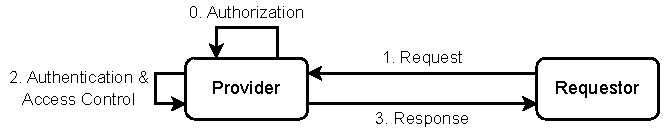
\includegraphics[width=0.9\textwidth]{./figures/access_control_request_traditional.drawio.pdf}
    \begin{redblock}{Problem}
        Too many provider responsibilities
        \\$\rightarrow$ Policy Management/Decisions/Enforcement, Request Verification, \& Response Creation
    \end{redblock}
\end{frame}
\begin{frame}{Attribute-Based Access Control (ABAC)}
    \begin{greenblock}{Definition \parencite{JTF2020}}
        Access control model enabling access decisions based on attributes associated with \textbf{subjects}, \textbf{objects}, \textbf{actions}, and the \textbf{environment} of a system.
    \end{greenblock}

    \begin{blueblock}{Discussion \parencite{Hu2014}}
        \begin{itemize}
            \item Multifactor Policy Expression $\rightarrow$ Fine-Grained \& Flexible Access Control (cf. RBAC/IBAC)
            \item Dynamic Policy Evaluation $\rightarrow$ Dynamic Authorization \& Real-Time Attributes
        \end{itemize}
    \end{blueblock}

    \begin{grayblock}{Architecture \parencite{Hu2014,Oasis2013}}
        \begin{itemize}
            \item Policy Decision Point (PDP) $\rightarrow$ Computes access decisions by evaluating policies
            \item Policy Enforcement Point (PEP) $\rightarrow$ Enforces policy decisions by controlling access to protected objects
        \end{itemize}
    \end{grayblock}
    % ABAC Definition
    % ABAC Benefit vs. traditional IBAC/RBAC solutions including RT-Attribute like network congestion
    % ABAC Requirements -> Authentication \& Authorization
\end{frame}
\begin{frame}{Server-Aided ABAC}
    \centering
    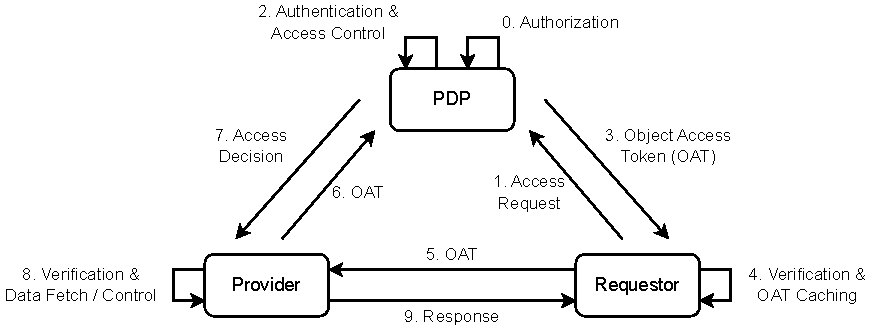
\includegraphics[width=1.0\textwidth]{./figures/access_control_request_delegation.drawio.pdf}
\end{frame}

\begin{frame}[allowframebreaks]{References}
\printbibliography
\end{frame}

\backupend

\end{document}